\documentclass[10pt,a4paper]{article}
\usepackage[margin=1.9cm,top=1.7cm,bottom=1.8cm]{geometry}
\usepackage[T1]{fontenc}
\usepackage{lmodern}
\renewcommand{\familydefault}{\sfdefault}
\usepackage{xcolor}
\usepackage{graphicx}
\usepackage{booktabs,tabularx,array,colortbl,longtable,needspace}
\usepackage{enumitem}
\usepackage{tikz}
\usetikzlibrary{arrows.meta,positioning,shapes.geometric,fit,calc,backgrounds}
\usepackage{titlesec}
\usepackage{fancyhdr}
\usepackage{caption}
\usepackage[hidelinks]{hyperref}

\definecolor{brand}{HTML}{B71C1C}
\definecolor{brandDark}{HTML}{7F0F0F}
\definecolor{brandTint}{HTML}{FBEAE8}
\definecolor{ink}{HTML}{1B1B1B}
\definecolor{muted}{HTML}{6B6B6B}
\definecolor{rule}{HTML}{E3C9C6}
\color{ink}

\titleformat{\section}{\large\bfseries\color{brand}}{\thesection}{0.6em}{}[{\color{rule}\titlerule}]
\titleformat{\subsection}{\normalsize\bfseries\color{brandDark}}{}{0pt}{}
\titlespacing*{\section}{0pt}{11pt}{5pt}
\titlespacing*{\subsection}{0pt}{7pt}{2pt}
\setlength{\parindent}{0pt}
\setlength{\parskip}{3.5pt}
\setlist{nosep,leftmargin=1.1em,itemsep=1.5pt}
\captionsetup{font={small,color=muted},labelfont={bf,color=brand},skip=3pt}
\renewcommand{\arraystretch}{1.18}
\pagestyle{fancy}
\fancyhf{}
\renewcommand{\headrulewidth}{0pt}
\fancyfoot[L]{\small\color{muted}Team Linear Regression}
\fancyfoot[R]{\small\color{muted}\thepage}
\newcommand{\tag}[1]{\textcolor{brand}{\textbf{#1}}}
\newcommand{\code}[1]{\texttt{\small #1}}
\newcolumntype{Y}{>{\raggedright\arraybackslash}X}
\newcommand{\HC}[1]{\textcolor{white}{\textbf{#1}}}
\newcolumntype{L}[1]{>{\raggedright\arraybackslash}p{#1}}

\begin{document}

% ------------------------------------------------------------------ title block
\noindent

\begin{tikzpicture}
  \fill[brand] (0,0) rectangle (\textwidth,3.05);
  \fill[brandDark] (0,0) rectangle (0.28,3.05);
  \node[anchor=north west,text=white,align=left,inner sep=0] at (0.7,2.75)
    {\Large\bfseries MEETING INTELLIGENCE ASSISTANT\\[3pt]\normalsize From a recorded meeting to a verified, structured record\\[7pt]
     \small\textbf{Team Linear Regression}\quad Akansha Das \;\textperiodcentered\; Atrijo Pal \;\textperiodcentered\; Anuj Sharma\\[2pt]
     \small Inter IIT Bootcamp, ML Problem Statement, Phase 2 \;\textperiodcentered\; Source: \href{https://github.com/atrijopal/boot}{\textcolor{white}{\underline{github.com/atrijopal/boot}}}};
\end{tikzpicture}

\section{What the system does}
The application takes an English meeting recording and, in one run, produces the five outputs the problem statement requires: a \tag{raw transcript}, a \tag{refined transcript}, \tag{meeting minutes}, a list of \tag{key decisions} and a list of \tag{action items}. Raw and refined transcripts are kept separately and compared in the interface. Every statement in the record is traceable to a quote, a speaker and a time in the recording. Where the meeting did not state an owner or a deadline, the record says \emph{unspecified}; a proposal is never reported as a decision, and an unstated assignment is never reported as a confirmed task.

\begin{tabularx}{\textwidth}{@{}>{\bfseries\raggedright\arraybackslash}p{2.9cm}Y L{4.7cm}@{}}
\rowcolor{brand}\HC{Output}&\HC{Content (from the brief)}&\HC{Where it is produced and exported}\\
Raw transcript & Speech-to-text result before language-model refinement & Transcript tab, TXT and JSON\\
\rowcolor{brandTint}Refined transcript & After domain-aware terminology correction; every change listed & Refinement tab, TXT and JSON\\
Meeting minutes & Concise summary and organised account of the discussion & Report: summary, topics. PDF, Markdown, HTML\\
\rowcolor{brandTint}Key decisions & Decisions reached; an empty list if none & Report and record JSON (\code{decisions})\\
Action items & Task, stated owner or deadline, otherwise \emph{unspecified} & Report, record JSON, CSV, ICS calendar\\
\end{tabularx}

The human-readable record (PDF, Markdown, HTML) and the machine-readable record (JSON, schema \code{meeting-record/1}) are generated from one structure, so both carry identical decisions and tasks; this is enforced by tests.

\section{Architecture}
The pipeline is a \tag{LangGraph} state machine with four nodes in the order the brief prescribes: transcription, speaker identification, refinement (language-model role~1) and documentation (language-model role~2). The two language-model roles are separate stages with separate prompts, models and outputs.
The backend owns the state: each meeting has a persisted session file with an explicit state per stage (\code{waiting}, \code{processing}, \code{needs\_review}, \code{completed}, \code{failed}). The interface only reads it. Two stages end in a human checkpoint (speakers, refinement) where the graph halts and resumes when the user approves; a failed stage can be retried alone, keeping earlier work.

\begin{figure}[h]
\centering
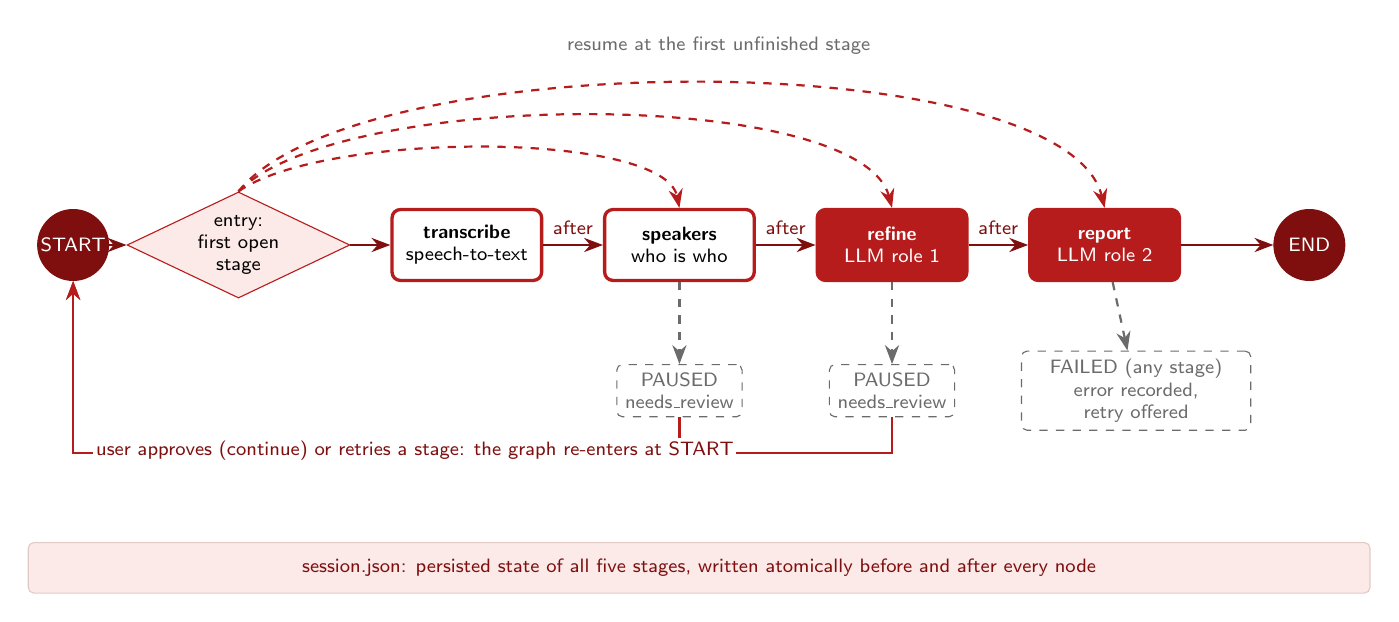
\begin{tikzpicture}[
  >={Stealth[length=2.4mm]}, font=\scriptsize,
  term/.style={circle,draw=brandDark,fill=brandDark,text=white,minimum size=9mm,inner sep=0},
  router/.style={diamond,aspect=2.1,draw=brand,fill=brandTint,inner sep=1pt,align=center},
  stage/.style={rounded corners=3pt,draw=brand,fill=white,very thick,minimum width=19mm,minimum height=9mm,align=center},
  llm/.style={rounded corners=3pt,draw=brand,fill=brand,text=white,very thick,minimum width=19mm,minimum height=9mm,align=center},
  stop/.style={rounded corners=2pt,draw=muted,dashed,fill=white,align=center,inner sep=3pt,text=muted},
  flow/.style={->,thick,color=brandDark},
  cond/.style={->,thick,color=brand,dashed}]
  \node[term] (s) at (0,0) {START};
  \node[router] (e) at (2.1,0) {entry:\\first open\\stage};
  \node[stage] (t) at (5.0,0) {\textbf{transcribe}\\speech-to-text};
  \node[stage] (sp) at (7.7,0) {\textbf{speakers}\\who is who};
  \node[llm] (r) at (10.4,0) {\textbf{refine}\\LLM role 1};
  \node[llm] (d) at (13.1,0) {\textbf{report}\\LLM role 2};
  \node[term] (en) at (15.7,0) {END};
  \draw[flow] (s) -- (e);
  \draw[flow] (e) -- (t);
  \draw[flow] (t) -- node[above]{after} (sp);
  \draw[flow] (sp) -- node[above]{after} (r);
  \draw[flow] (r) -- node[above]{after} (d);
  \draw[flow] (d) -- (en);
  % resume edges from the entry router
  \draw[cond] (e.north) .. controls (3.2,1.45) and (7.5,1.45) .. (sp.north);
  \draw[cond] (e.north) .. controls (3.4,2.0) and (10.0,2.0) .. (r.north);
  \draw[cond] (e.north) .. controls (3.6,2.55) and (12.6,2.55) .. (d.north);
  \node[above,text=muted] at (8.2,2.3) {resume at the first unfinished stage};
  % pauses
  \node[stop] (p1) at (7.7,-1.85) {PAUSED\\needs\_review};
  \node[stop] (p2) at (10.4,-1.85) {PAUSED\\needs\_review};
  \node[stop,text width=27mm] (f) at (13.5,-1.85) {FAILED (any stage)\\error recorded, retry offered};
  \draw[cond,color=muted] (sp) -- (p1);
  \draw[cond,color=muted] (r) -- (p2);
  \draw[cond,color=muted] (d) -- (f);
  \draw[->,thick,color=brand] (p1.south) -- ++(0,-0.45) -| (s.south);
  \draw[->,thick,color=brand] (p2.south) -- ++(0,-0.45) -| (s.south);
  \node[fill=white,text=brandDark,inner sep=1pt,anchor=south west] at (0.25,-2.78) {user approves (continue) or retries a stage: the graph re-enters at START};
  % session file
  \begin{scope}[on background layer]
  \node[draw=rule,fill=brandTint,rounded corners=2pt,fit={(-0.5,-4.35) (16.4,-3.85)},inner sep=2pt] (ses) {};
  \end{scope}
  \node[text=brandDark] at (7.95,-4.1) {session.json: persisted state of all five stages, written atomically before and after every node};
\end{tikzpicture}
\caption{LangGraph state machine. Solid arrows are the normal flow; dashed arrows are conditional routes decided from the persisted session.}
\end{figure}

\begin{figure}[h]
\centering
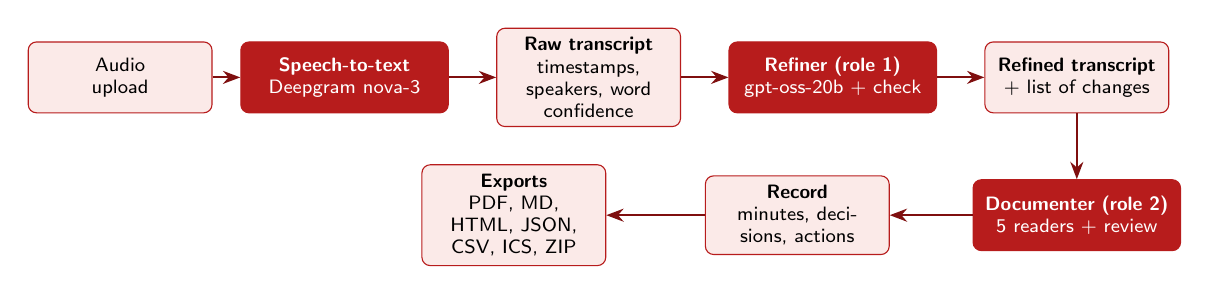
\begin{tikzpicture}[>={Stealth[length=2.2mm]},font=\scriptsize,
  box/.style={rounded corners=3pt,draw=brand,fill=brandTint,minimum height=9mm,align=center,text width=21mm},
  mod/.style={rounded corners=3pt,draw=brand,fill=brand,text=white,minimum height=9mm,align=center,text width=24mm},
  a/.style={->,thick,color=brandDark}]
  \node[box] (au) at (0,0) {Audio\\upload};
  \node[mod] (asr) at (2.85,0) {\textbf{Speech-to-text}\\Deepgram nova-3};
  \node[box] (raw) at (5.95,0) {\textbf{Raw transcript}\\timestamps, speakers, word confidence};
  \node[mod] (ref) at (9.05,0) {\textbf{Refiner (role 1)}\\gpt-oss-20b + check};
  \node[box] (rf) at (12.15,0) {\textbf{Refined transcript}\\+ list of changes};
  \node[mod] (doc) at (12.15,-1.75) {\textbf{Documenter (role 2)}\\5 readers + review};
  \node[box] (rec) at (8.6,-1.75) {\textbf{Record}\\minutes, decisions, actions};
  \node[box] (ex) at (5.0,-1.75) {\textbf{Exports}\\PDF, MD, HTML, JSON, CSV, ICS, ZIP};
  \draw[a](au)--(asr); \draw[a](asr)--(raw); \draw[a](raw)--(ref); \draw[a](ref)--(rf); \draw[a](rf)--(doc); \draw[a](doc)--(rec); \draw[a](rec)--(ex);
\end{tikzpicture}
\caption{How outputs move between stages. The documenter reads the \emph{refined} transcript, never the raw one.}
\end{figure}

\section{Models and fallbacks}
\begin{tabularx}{\textwidth}{@{}L{3.2cm}L{4.1cm}Y@{}}
\rowcolor{brand}\HC{Role}&\HC{Model}&\HC{Purpose}\\
Speech-to-text & Deepgram \textbf{nova-3} & Whole file in one request; word timestamps, confidences and \emph{voice-based} speaker labels\\
\rowcolor{brandTint}Speech-to-text (alt.) & Groq \textbf{whisper-large-v3}, 10-min chunks & Used when no Deepgram key is set; text only, no speakers\\
Role 1: proposer & \textbf{gpt-oss-20b} (reasoning: medium) & Proposes small exact fixes to terms, acronyms, names\\
\rowcolor{brandTint}Role 1: second check & \textbf{qwen3.8-27b} (low) & Different model family confirms or rejects a fix that has no support in the recording\\
Speaker names & \textbf{gpt-oss-20b} (low) & Suggests a name or role only with a quote that shows it\\
\rowcolor{brandTint}Role 2: readers & \textbf{qwen3.8-27b} $\times$4, \textbf{gpt-oss-120b} $\times$1 & Five focused readers (see below); the 120b reads tasks, owners and deadlines, the error-prone part\\
Role 2: review & \textbf{gpt-oss-120b} (low) & Checks decisions and tasks, writes headline, summary, topic bullets\\
\end{tabularx}

\textbf{Why several models.} Each call uses the smallest model and reasoning effort that does its job, and the review model is a different family from most readers, so it checks them independently rather than repeating their mistakes.

\textbf{Fallbacks.} (1) A language-model call that is refused or unavailable is answered by a configured backup model (\code{FALLBACK\_MODEL}, NVIDIA nemotron-3-super-120b); both attempts remain visible in the audit view. (2) A speech-to-text chunk falls back from whisper-large-v3 to whisper-large-v3-turbo; the provider is chosen automatically (Deepgram if configured). (3) An unreadable JSON answer is retried, once with lower reasoning effort. (4) If the review cannot run, the report is still produced from the verified records, the summary is restated from verbatim quotes, and every decision is tagged \emph{not confirmed} with a banner and a ``run the final check again'' action. (5) A failed stage is retried alone; finished stages are kept.

\section{Prompts}
All 13 prompts are stored as files in \code{prompts/} and are the only model instructions. Each treats the transcript as delimited data (a prompt-injection firewall), demands JSON only, and states what must \emph{not} be done.
\begin{longtable}{@{}L{3.6cm}L{2.0cm}L{11.0cm}@{}}
\rowcolor{brand}\HC{Prompt}&\HC{Stage}&\HC{Instruction in brief}\\
\endhead
\code{refine} & Refinement & Return edits only (\code{find}, \code{rep}, kind), never rewritten text; fix terms, acronyms, names, spelling; never touch numbers, dates, negations or commitments\\
\rowcolor{brandTint}\code{verify\_edits} & Refinement & Same meaning? Anything new added? Reject if unsure\\
\code{names} & Speakers & Name or role only from self-introduction or being addressed and answering; quote required\\
\rowcolor{brandTint}\code{speakers} & Speakers & Optional text-only speaker labelling (off by default; measured unreliable)\\
\code{extract\_decisions} & Report & Decisions and proposals; a proposal is not a decision\\
\rowcolor{brandTint}\code{extract\_actions} & Report & Tasks; owner only if the speaker commits in first person or is named; deadline only if quoted\\
\code{extract\_issues} & Report & Questions, concerns, risks, disagreements\\
\rowcolor{brandTint}\code{extract\_details} & Report & Figures, topics, names\\
\code{extract\_discussion} & Report & Main discussion points\\
\rowcolor{brandTint}\code{extract\_core}, \code{extract\_context}, \code{extract} & Report & Two-reader and single-reader variants used when a long meeting must fit a call budget\\
\code{review} & Report & Verdicts that can only remove or weaken a record; headline, summary citing record ids, topic bullets, per-speaker summaries\\
\end{longtable}

\subsection{Safeguards implemented in code (no model involved)}
\begin{itemize}
\item A quote must appear \emph{word for word} in the transcript; a quote may not skip a negation; a number in a record must be in its quote.
\item A correction may not touch a number, date, time, duration or negation, may not overlap them, and is size-limited; the check re-runs the extractors on the edited text.
\item A correction is applied automatically only if the recording supports it (same word elsewhere, the recogniser's own alternative) or the independent second check confirms it; otherwise it is only \emph{suggested}.
\item Owner: first-person commitment by a labelled speaker, or named in the quote; deadline: only if quoted; otherwise \emph{unspecified}.
\item Every summary sentence must cite kept records and add no new number; duplicate records from overlapping windows are merged.
\item The server re-validates every correction a user accepts; speaker names are shown only when the meeting shows them or the user types them.
\end{itemize}

\section{Token efficiency}
\begin{enumerate}[label=\textbf{\arabic*.}]
\item \textbf{Compact encoding:} transcript lines as \code{u012 A: text}, short consecutive lines of one speaker merged, short JSON keys.
\item \textbf{Code does the cheap work:} numbers, dates, durations, negations, acronyms and rare words are found by code and pre-flagged, so the model does not hunt for them.
\item \textbf{Edit-only refinement:} the model returns a few \code{find}/\code{rep} pairs, not the transcript.
\item \textbf{The review reads records, not the transcript} (about 4k tokens instead of the full text).
\item \textbf{Windowing:} about 3,500 transcript tokens per call; a hard call cap (6) makes windows grow or readers merge rather than the cost grow.
\item \textbf{Right-sized models and effort:} low effort for narrow tasks; the 120b only for owners/deadlines and the review.
\item \textbf{Second check only when needed:} only for suggested fixes without evidence in the recording.
\item \textbf{Budgets:} 7,000 tokens per call and 80,000 per run; a run that would exceed them is refused with a clear message before it starts.
\item \textbf{Content-addressed cache and stage retry:} identical inputs cost zero tokens; a retry re-runs only the failed stage.
\end{enumerate}

\textbf{Measured on a 5-minute meeting (full run, all stages completed):}
\begin{center}
\begin{tabularx}{0.96\textwidth}{@{}Y r r L{4.6cm} r@{}}
\rowcolor{brand}\HC{Stage}&\HC{Calls}&\HC{Tokens}&\HC{Model(s)}&\HC{Share}\\
Speaker names & 1 & 1,757 & gpt-oss-20b & 8\%\\
\rowcolor{brandTint}Refinement (+ check) & 1 & 3,531 & gpt-oss-20b / qwen & 16\%\\
Five readers & 5 & 11,873 & qwen $\times$4, 120b & 55\%\\
\rowcolor{brandTint}Review and summary & 1 & 4,270 & gpt-oss-120b & 20\%\\
\textbf{Total} & \textbf{8} & \textbf{21,431} & 20b 25\%, qwen 41\%, 120b 35\% & \\
\end{tabularx}
\end{center}
That is about \textbf{4.3k tokens per minute of audio} and a mean of about 2.7k tokens per call. The readers scale with length (17.1k for a 7.5-minute meeting against 11.9k for 5 minutes) while the review stays near 4--6k. Splitting extraction into focused readers raised the number of verified records on the same 12-minute clip from 3--5 to 12--13 for roughly 4--5k extra tokens.

\section{Interface}
The interface follows the workflow: Upload, Speakers, Transcript, Refinement, Meeting report, Export, plus a Pipeline tab that shows what each stage received and returned. A stage bar shows status at all times, with plain-language errors and a retry button for a failed stage.
\begin{itemize}
\item \textbf{Upload:} WAV, MP3, M4A, FLAC, OGG, OPUS, WebM, AAC; unsupported, empty, silent, corrupt or too-short files are rejected with an explanation.
\item \textbf{Speakers:} suggested names with their evidence quote; accept, edit, or leave a speaker unnamed.
\item \textbf{Transcript:} raw and refined views, search with highlighting, speaker filter, click a timestamp to play the real recording from that point, copy and download.
\item \textbf{Refinement review:} original, proposed text, reason and evidence for every change; accept, reject, accept all, filters, side-by-side view.
\item \textbf{Report:} a numbered document; every item links to its line in the transcript; \emph{Unspecified} for missing owners and deadlines; uncertainty listed with severity (info, review, warning, error).
\item \textbf{Export:} only files that exist are offered, with professional names; a ZIP bundles them with a manifest.
\end{itemize}

\begin{figure}[h]
\centering
\begin{minipage}[b]{0.545\textwidth}\centering
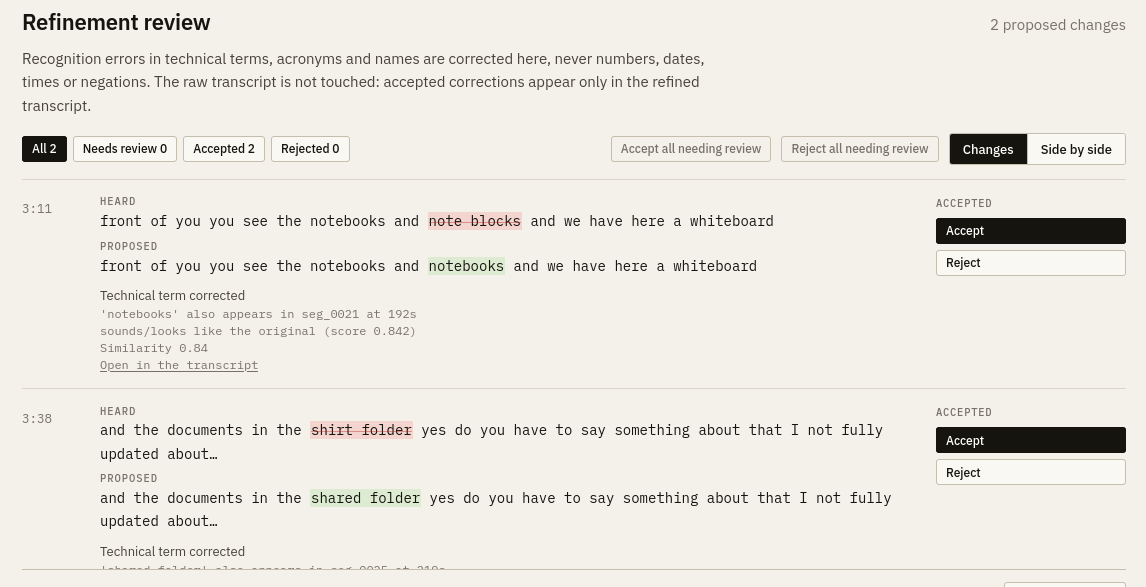
\includegraphics[height=4.7cm]{figures/refinement_crop.png}
\captionof{figure}{Refinement review: each proposed change with its evidence.}
\end{minipage}\hfill
\begin{minipage}[b]{0.43\textwidth}\centering
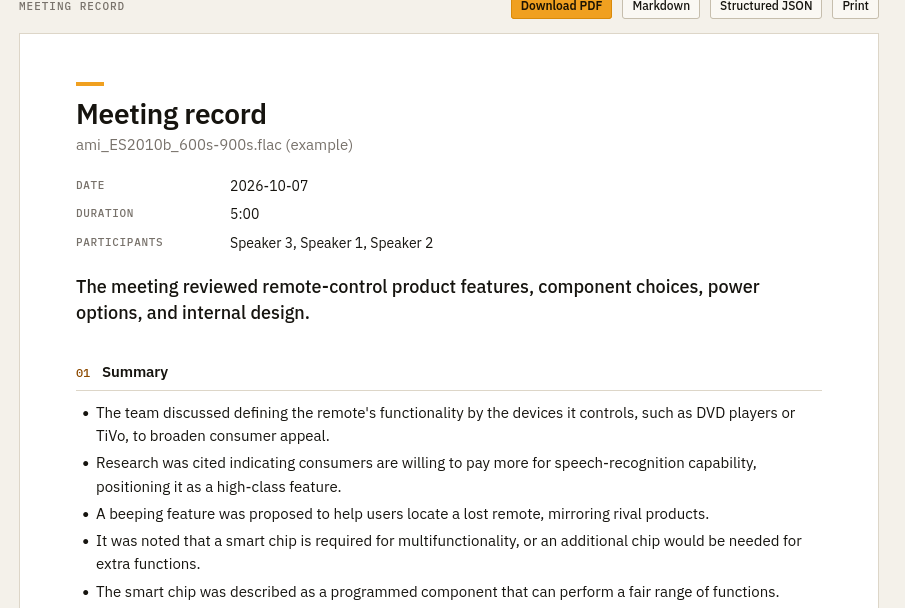
\includegraphics[height=4.7cm]{figures/report_crop.png}
\captionof{figure}{Meeting record: every item carries its source.}
\end{minipage}
\end{figure}

\begin{figure}[h]
\centering
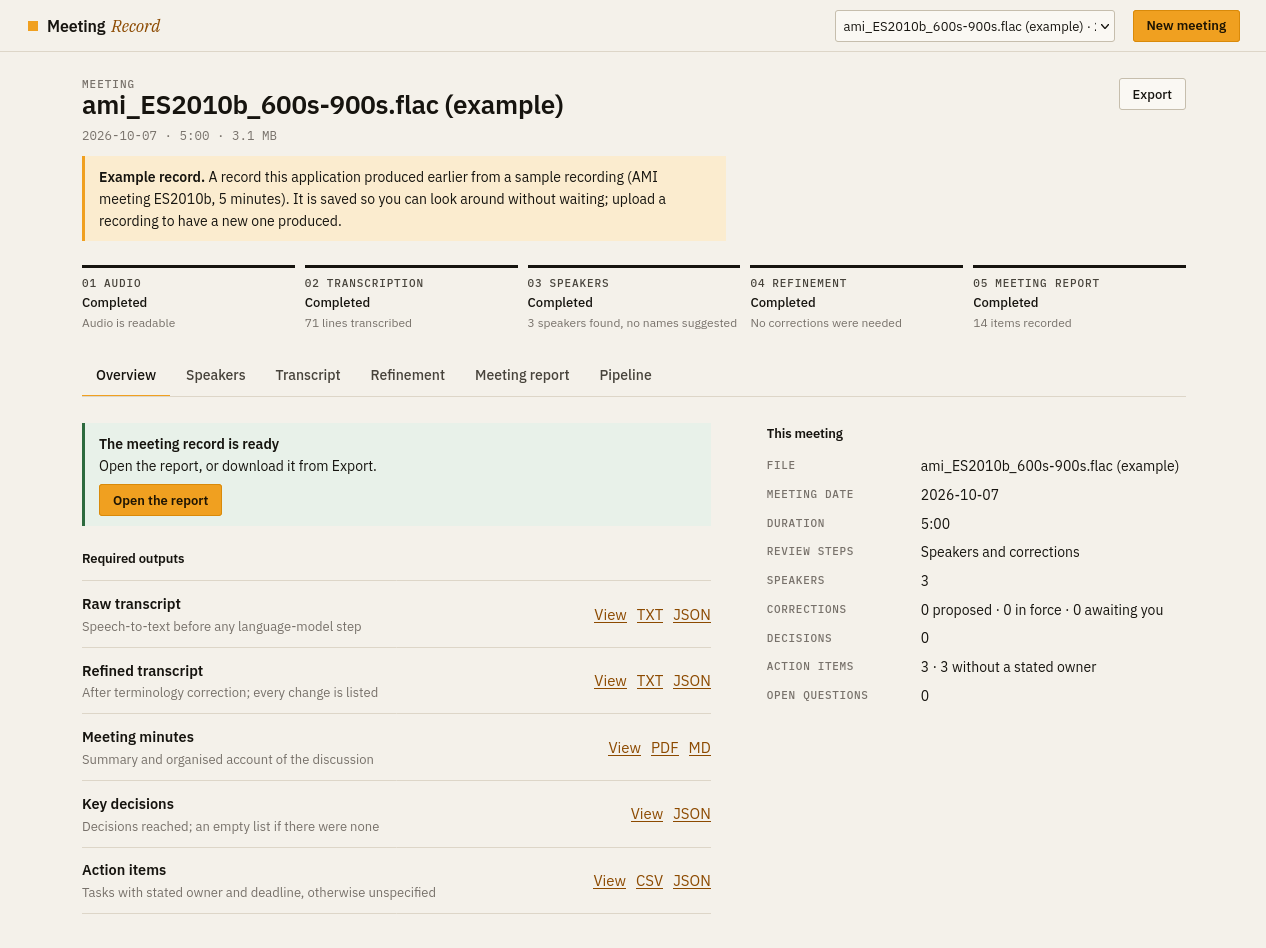
\includegraphics[width=0.74\textwidth]{figures/overview.png}
\caption{Overview: stage status, next step, and the five required outputs, each with a view link and downloads.}
\end{figure}

\Needspace{9\baselineskip}
\section{Evaluation}
Ground truth comes from the public human transcripts and annotations of the AMI Meeting Corpus (CC BY 4.0); the repository provides scripts to build a reference for any clip and score a run (\code{scripts/make\_reference.py}, \code{scripts/evaluate.py}).
\begin{center}
\begin{tabularx}{0.98\textwidth}{@{}Y l l@{}}
\rowcolor{brand}\HC{Measurement (12-minute clips, single runs)}&\HC{Result}&\HC{Reference}\\
Word error rate, Deepgram nova-3, quiet meeting (ES2002a) & 19.8\% & human transcript\\
\rowcolor{brandTint}Word error rate, Deepgram nova-3, loud office meeting (IB4001) & 25.4\% & human transcript\\
Word error rate, Groq whisper-large-v3, same office clip & 29.8\% & human transcript\\
\rowcolor{brandTint}Words given the correct speaker (4 real speakers found) & 95.7\% / 86.5\% & human labels\\
Speaker labels guessed from text alone & 28--40\% & chance level; switched off\\
\end{tabularx}
\end{center}
Most word errors are words lost where people talk over each other. Refinement was checked with planted terminology errors: 8 of 9 were corrected, and an earlier false correction of a person's name was removed by the stricter prompt and the second check. The suite contains \textbf{174 automated tests} that run offline with a faked recogniser and model: the gates, graph routing, session recovery, every export, error messages, and a scan proving no model name, token count or prompt text reaches a user-visible page or file.

\section{Deliverables and limits}
The repository contains the full application, all prompts, dependency list and a README with setup and run steps (\code{bash run.sh}); sample recordings with reference transcripts; and generated example outputs (raw and refined transcript, minutes, decisions, action items) in \code{samples/example\_outputs/}. A saved example meeting is labelled as such and is never returned for a new upload: every new recording is processed by the pipeline.

\textbf{Limits.} English only. Language models can be wrong; the checks reduce this but do not prove correctness. Speaker separation needs the Deepgram provider. Long meetings beyond about 15 minutes have been exercised by tests with a fake model, not live. Source: \href{https://github.com/atrijopal/boot}{\textcolor{brand}{github.com/atrijopal/boot}}.

\end{document}
